\section{Dataflow Engine for Filtering and Dropping}
\label{sec:arch}

% % Overview of inserting dataflow engine between main and monitoring core
% \begin{figure}
%   \begin{center}
%     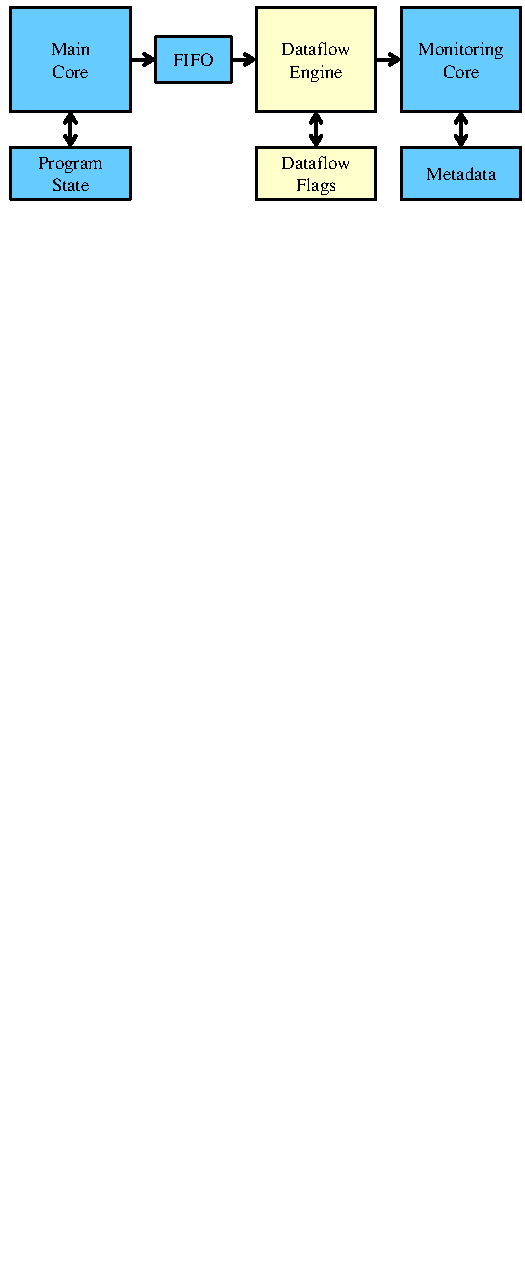
\includegraphics[width=\linewidth]{figs/dataflow_overview.pdf}
%     \vspace{-0.2in}
%     \caption{Overview of architecture for reduced and adjustable monitoring
%     overheads.}
%     \label{fig:arch.overview} 
%     \vspace{-0.1in}
%   \end{center}
% \end{figure}

% Overview of full architecture
\begin{figure}
  \begin{center}
    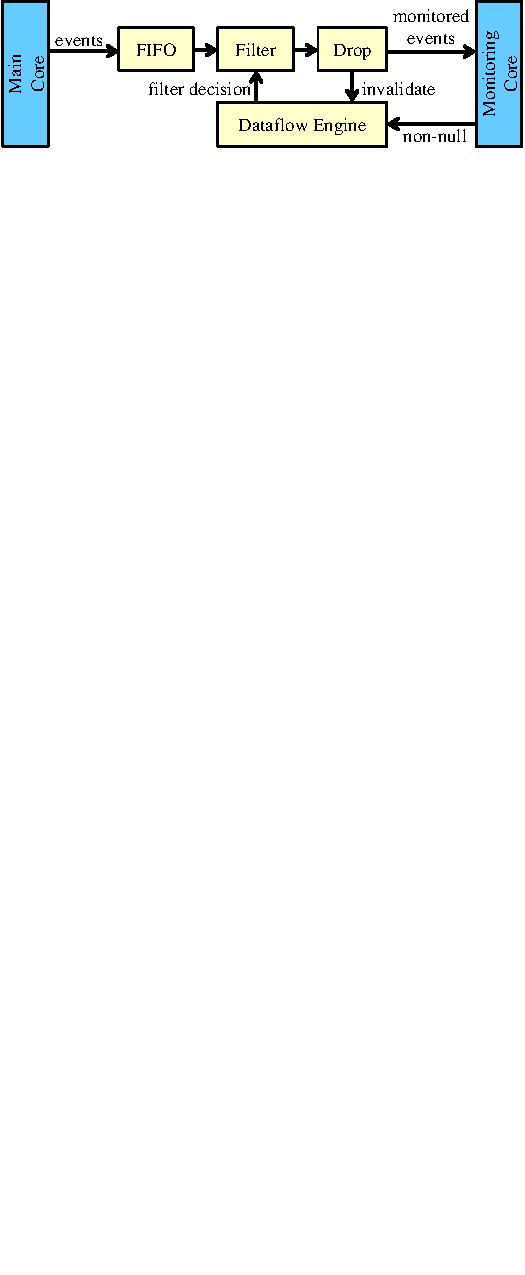
\includegraphics[width=\columnwidth]{figs/architecture_overview.pdf}
    \vspace{-0.2in}
    \caption{Block diagram of architecture for monitoring with reduced and adjustable overheads.}
    \label{fig:arch.overview}
    \vspace{-0.1in}
  \end{center}
\end{figure}

For both filtering and partial monitoring, we need to be able to track
dataflows. For filtering, we need to track the dataflow of null metadata and
for partial monitoring, we need to track the dataflow of invalid metadata.
In this section, we will describe our dataflow-guided hardware architecture for
enabling both filtering and partial monitoring.
Figure~\ref{fig:arch.overview} shows a high-level block diagram of the
architecture. The basic idea is to insert this dataflow-guided hardware between the main core and
the monitoring core that will reduce the number of monitoring events that reach
the monitoring core and thus reduce the overheads of monitoring.

As in the baseline architecture from Section~\ref{sec:monitoring}, events from
the main core are first buffered in a FIFO. 
Events are first filtered out based on whether they correspond to null or
invalid metadata. A hardware dataflow engine is used to track the flow of null
and invalid metadata and decide whether
specific events can be filtered out.
Next, if the event is not filtered out, then we
check whether the event should be dropped in order to stay within the specified
overhead budget. Whenever an event is dropped, its corresponding metadata is
marked and tracked as invalid by the dataflow engine. The
dropping decision hardware is described in detail in Section~\ref{sec:policies}.
Finally, if the event is not filtered or dropped, then it is forwarded to the
monitoring core to be processed.

\subsection{Filtering Using the Dataflow Engine}
\label{sec:arch.dataflow}

% Detailed architecture of dataflow engine
\begin{figure*}
  \begin{center}
    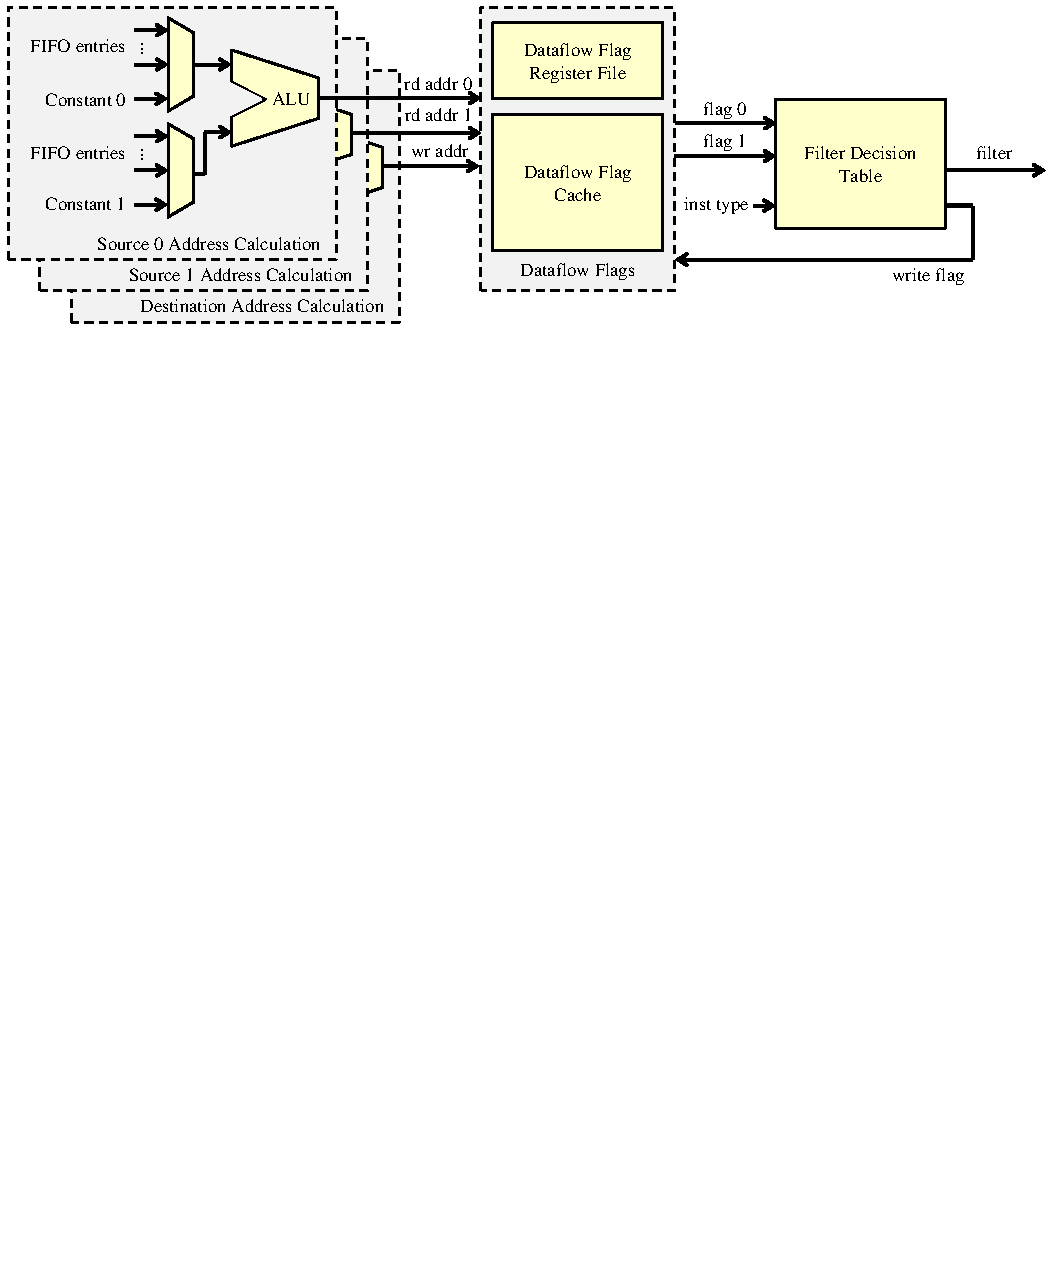
\includegraphics[width=\linewidth]{figs/dataflow_architecture.pdf}
    \vspace{-0.2in}
    \caption{Hardware architecture of the dataflow engine.}
    \label{fig:arch.dataflow} 
    \vspace{-0.1in}
  \end{center}
\end{figure*}

% Overview
In order to perform filtering, we need to be able to identify and track flows
of null metadata. Similarly, for partial monitoring,
 we need to be able to track the flow of invalid metadata. In
order to efficiently these flows, we use a dedicated hardware
dataflow engine. A block diagram of the dataflow engine is shown in
Figure~\ref{fig:arch.dataflow}.

% Flags and flag storage
In order track both null metadata flows and invalid metadata flows, the
dataflow engine tracks the flow of 2-bit flags. One bit is used to
mark metadata as null while the other bit is used to mark metadata as invalid.
Monitoring schemes typically keep metadata corresponding to the main core's
register file as well as the main core's memory space. Similarly, the dataflow
engine uses an on-chip register file to store flags for register file metadata.
In addition, a set of flags are stored that correspond to memory metadata.
These memory metadata flags are accessed through a cache and backed to main
memory. All flags are initialized as null and valid when the system starts. 

% Address calculation and configuration
On a monitoring event, the dataflow engine reads in up to two flags in order to
determine whether the event can be filtered.  The flags to be read in typically correspond to the source
operands of the monitored instruction. For example, on a load, the dataflow
engine will typically read in the flags corresponding the memory location
accessed.
However, the architecture is designed such that the address of flags to be read
is calculated dynamically and can be configured depending on the monitoring
scheme. Specifically, there exists a configuration table that outputs a set of
control signals depending on the instruction type of the monitoring event.
These control signals are used to control a pair of address calculation units which each
contain a simple ALU. The inputs to the ALU are information from the monitored
event and a constant that is specified from the configuration table. One common
use of this address calculation is to transform addresses from byte-addressed
to word-addressed by right shifting the passed memory address by 2 bits.

% Filtering decision
The decision of whether an event can be filtered out is determined using a
lookup table. This filter decision table is configured by the monitoring scheme
on system initialization. The lookup table determines whether an event can be
filtered out based on the pair of input flags read and the instruction type of
the monitored event.
For example, on an ALU instruction, if both of the source operand flags
indicate that the corresponding metadata is null, then typically the instruction can be
filtered out. Similarly, on an ALU instruction, if either of the source operand
flags indicate that their corresponding metadata is invalid, then the
instruction can also be filtered out. This filter decision is sent to the
``Filter'' block shown in Figure~\ref{fig:arch.overview} which will simply pop
filtered entries from the FIFO and not forward them. If an entry is not
filtered, then this Filter block will pop the monitoring event entry from the
FIFO and forward it along the datapath.

% Propagating flag information
Finally, when an event is filtered out, it is necessary to propagate the flag
information for the filtered event. In addition to the decision of whether to
filter an event, the filter decision table also includes information about
whether the destination flag should be written to and what value should be
written to it. A third address calculation unit generates the write address for
this destination flag. For example, for an ALU instruction, this will
correspond to the destination register of the ALU instruction. If this ALU
instruction is filtered out due to having a pair of null source operands, then
the filter decision table will indicate that the destination register's
corresponding flag should also be marked as null. 

\subsection{Setting Dataflow Flags}
\label{sec:arch.dropping}

Although the dataflow engine automatically propagates information about
non-null and invalid metadata, it also requires for these flows to be
initialized. That is, there needs to be some way to mark metadata as non-null
or invalid. These interfaces from the monitoring core and the dropping hardware
are marked in Figure~\ref{fig:arch.overview}.

Metadata is marked as non-null when the monitoring core writes a valid metadata
value. When the monitoring core performs these metadata update operations, it
also writes to the corresponding dataflow flag to mark the flag as non-null.

Flags are marked as invalid when a monitoring event is dropped due to
insufficient overhead budget. Thus, whenever a monitoring event is dropped, the
dropping hardware indicates this to the dataflow engine. The dataflow engine's
write address is configured for the appropriate destination flag. When it
receives an invalidation signal from the dropping hardware, the
dataflow engine marks this destination flag as invalid.

\subsection{Example Extensions}
